% Chapter 6. cacheScope is an access-control decision wearing performance clothing.
\documentclass[tikz,border=6pt]{standalone}
% Shared look for every TikZ figure in the book.
% Colours match book/preamble.tex exactly. Change both or neither.

\usepackage{tikz}
\usepackage{xcolor}
\usepackage{amsmath}
\IfFileExists{libertinus.sty}{\usepackage[mono=false]{libertinus}}{}
\IfFileExists{inconsolata.sty}{\usepackage[varqu,varl,scaled=0.95]{inconsolata}}{}

\usetikzlibrary{
  arrows.meta, positioning, calc, fit, backgrounds, shapes.geometric,
  shapes.misc, decorations.pathreplacing, decorations.pathmorphing,
  patterns, chains, matrix, shadows.blur
}

\definecolor{ink}{HTML}{15181D}
\definecolor{muted}{HTML}{5B6472}
\definecolor{rule}{HTML}{C9CED6}
\definecolor{wash}{HTML}{F4F5F7}
\definecolor{accent}{HTML}{0F5C8C}
\definecolor{accentsoft}{HTML}{E7F0F6}
\definecolor{warm}{HTML}{B4531A}
\definecolor{warmsoft}{HTML}{FBF0E7}
\definecolor{good}{HTML}{2C6E49}
\definecolor{goodsoft}{HTML}{E9F2EC}
\definecolor{danger}{HTML}{9B2226}
\definecolor{dangersoft}{HTML}{FAECEC}

\tikzset{
  font=\sffamily\small,
  >={Stealth[length=5pt, width=4pt]},
  %
  box/.style={
    draw=rule, line width=0.8pt, fill=wash, rounded corners=2pt,
    inner sep=7pt, align=center, text=ink, minimum height=9mm,
  },
  boxa/.style={box, draw=accent, fill=accentsoft},
  boxg/.style={box, draw=good,   fill=goodsoft},
  boxw/.style={box, draw=warm,   fill=warmsoft},
  boxd/.style={box, draw=danger, fill=dangersoft},
  %
  lane/.style={draw=rule, line width=0.7pt, fill=white, rounded corners=2pt,
               inner sep=6pt, align=center, minimum width=26mm},
  %
  flow/.style={draw=accent, line width=1.0pt, ->},
  flowback/.style={flow, densely dashed},
  flowmuted/.style={draw=muted, line width=0.8pt, ->},
  lifeline/.style={draw=rule, line width=0.7pt, densely dotted},
  %
  lbl/.style={font=\sffamily\scriptsize, text=muted, inner sep=2pt},
  lblink/.style={font=\sffamily\scriptsize, text=ink, inner sep=2pt},
  tag/.style={font=\ttfamily\scriptsize, text=accent, inner sep=2pt,
              fill=white, inner xsep=3pt},
  note/.style={font=\sffamily\scriptsize\itshape, text=muted, align=left},
  %
  band/.style={draw=none, rounded corners=1pt},
  tick/.style={draw=muted, line width=0.6pt},
}

% A horizontal timeline bar segment: \barseg{x0}{x1}{y}{colour}{label}
\newcommand{\barseg}[5]{%
  \fill[#4, rounded corners=1pt] (#1,#3-0.16) rectangle (#2,#3+0.16);
  \node[lbl, text=white, font=\sffamily\scriptsize\bfseries]
       at ({(#1+#2)/2},#3) {#5};
}

\begin{document}
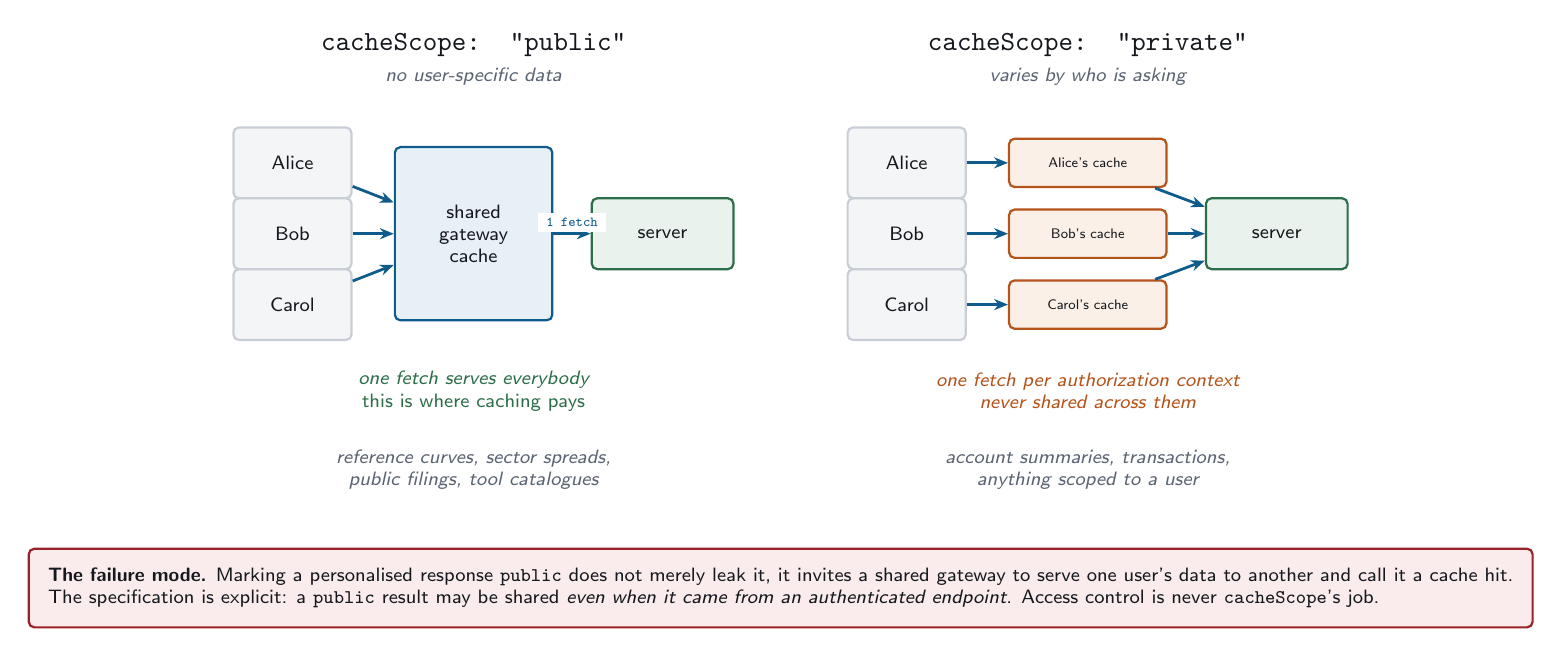
\begin{tikzpicture}[x=1cm, y=1cm]

% ---------------------------------------------------------------- public
\begin{scope}[xshift=0cm]
  \node[lblink, font=\sffamily\bfseries] at (2.6,3.5) {\texttt{cacheScope: "public"}};
  \node[note, align=center] at (2.6,3.1) {no user-specific data};

  \node[box, minimum width=15mm, font=\sffamily\scriptsize] (a1) at (0.3,2.0) {Alice};
  \node[box, minimum width=15mm, font=\sffamily\scriptsize] (b1) at (0.3,1.1) {Bob};
  \node[box, minimum width=15mm, font=\sffamily\scriptsize] (c1) at (0.3,0.2) {Carol};

  \node[boxa, minimum width=20mm, minimum height=22mm, align=center,
        font=\sffamily\scriptsize] (gw1) at (2.6,1.1) {shared\\gateway\\cache};

  \node[boxg, minimum width=18mm, font=\sffamily\scriptsize] (s1) at (5.0,1.1) {server};

  \foreach \x in {a1,b1,c1} { \draw[flow] (\x) -- (gw1); }
  \draw[flow] (gw1) -- node[tag, above, font=\ttfamily\tiny] {1 fetch} (s1);

  \node[note, align=center, text=good] at (2.6,-0.9)
    {one fetch serves everybody\\\emph{this is where caching pays}};
  \node[note, align=center, text=muted] at (2.6,-1.9)
    {reference curves, sector spreads,\\public filings, tool catalogues};
\end{scope}

% --------------------------------------------------------------- private
\begin{scope}[xshift=7.8cm]
  \node[lblink, font=\sffamily\bfseries] at (2.6,3.5) {\texttt{cacheScope: "private"}};
  \node[note, align=center] at (2.6,3.1) {varies by who is asking};

  \node[box, minimum width=15mm, font=\sffamily\scriptsize] (a2) at (0.3,2.0) {Alice};
  \node[box, minimum width=15mm, font=\sffamily\scriptsize] (b2) at (0.3,1.1) {Bob};
  \node[box, minimum width=15mm, font=\sffamily\scriptsize] (c2) at (0.3,0.2) {Carol};

  \node[boxw, minimum width=20mm, minimum height=6mm, font=\sffamily\tiny] (ca) at (2.6,2.0) {Alice's cache};
  \node[boxw, minimum width=20mm, minimum height=6mm, font=\sffamily\tiny] (cb) at (2.6,1.1) {Bob's cache};
  \node[boxw, minimum width=20mm, minimum height=6mm, font=\sffamily\tiny] (cc) at (2.6,0.2) {Carol's cache};

  \node[boxg, minimum width=18mm, font=\sffamily\scriptsize] (s2) at (5.0,1.1) {server};

  \draw[flow] (a2) -- (ca); \draw[flow] (b2) -- (cb); \draw[flow] (c2) -- (cc);
  \draw[flow] (ca) -- (s2); \draw[flow] (cb) -- (s2); \draw[flow] (cc) -- (s2);

  \node[note, align=center, text=warm] at (2.6,-0.9)
    {one fetch per authorization context\\never shared across them};
  \node[note, align=center, text=muted] at (2.6,-1.9)
    {account summaries, transactions,\\anything scoped to a user};
\end{scope}

% --------------------------------------------------------------- warning
\node[boxd, minimum width=150mm, align=left, font=\sffamily\scriptsize]
  at (6.5,-3.4)
  {\textbf{The failure mode.} Marking a personalised response \texttt{public}
   does not merely leak it, it invites a shared gateway to serve one user's
   data to another and call it a cache hit.\\
   The specification is explicit: a \texttt{public} result may be shared
   \emph{even when it came from an authenticated endpoint}. Access control is
   never \texttt{cacheScope}'s job.};

\end{tikzpicture}
\end{document}
